\section{Demonstration}
\label{sec:demo}

\ceg{Note this section will be spread out into the other sections.}

\system is demonstrated with the help of a web page which allows the user to perform exploratory search on DBLP conference's scientific papers \cite{Tang:2008:EMA:1367497.1367722}. All the searches in the system keep in account the user model. The user model is a profile of preference provided by the user before he makes any search. This is done by specifying weightage to various topics. The \system website has a list of topics with a slider associated with each of them using which a user can specify the degree of interest in that particular topic. This array of user preference is used as the ranking factor in all the results. The web site has three basic functionality which has been classified under three different tabs of the same name. They are keyword paper search, Topic explore, and Graph explore. 

\paragraph{Keyword Paper Explore} This is a universal search facility. The user may enter one or more keywords representing topics, or author names etc. The key words are searched in the title, abstract, and the author names of all the papers and are listed. The listing is ranked based on the user model. In the first page only a few of the papers are displayed  in two boxes - one containing matching words in the title, and the other in the abstract. Clicking on any box will open up a more complete list of papers.

\begin{figure}[htb]
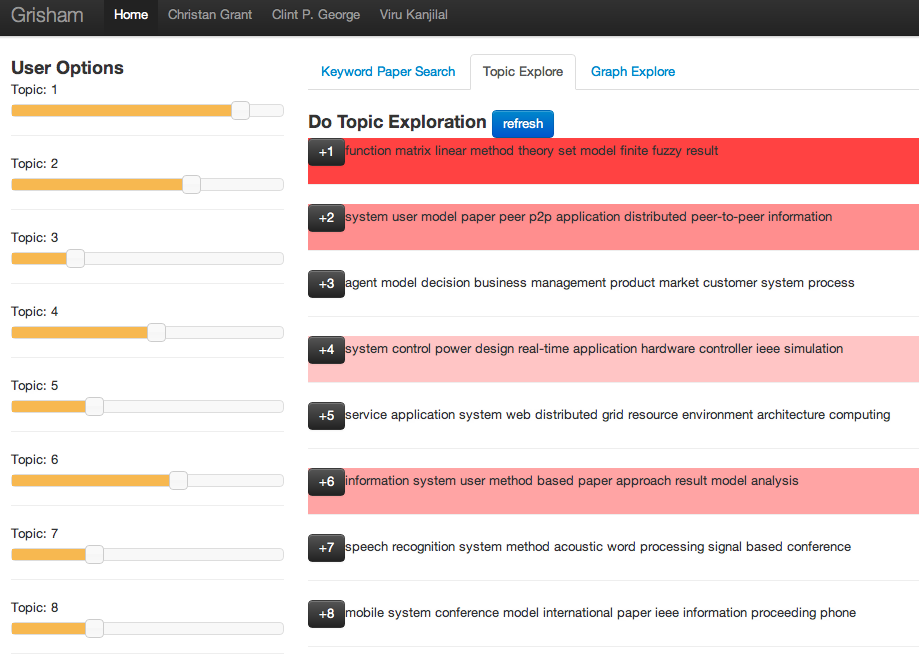
\includegraphics[width=.5\textwidth]{images/topic_exploration.png} % scale=.25,trim=0 0 300 0
\caption{User configured topic exploration}
\label{fig:topic_exploration}
\end{figure}

\paragraph{Topic Explore} The second tab on the website is for topic exploration and it allows a user to click on a specific topic to know more about the papers associated with the topic. Initially all the extracted topics from the corpus are shown along with their topic words. This list is color coded to distinguish the relevance of topics as indicated by the user model. The list is clickable and one a topic is clicked, relevant papers to that topic ranked based on the user model and displayed.
A screenshot is shown in figure~\ref{fig:topic_exploration}.

\begin{figure}[htb]\centering 
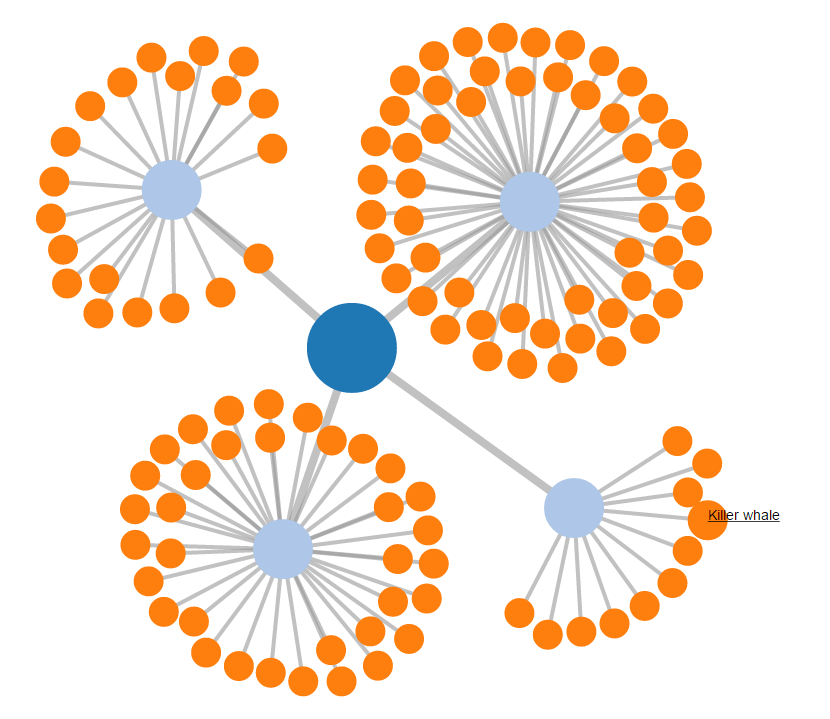
\includegraphics[width=.5\textwidth]{images/topical_docs.png}
\caption{Visualizing of Topic-Based Search in \system, orange 
circles represent documents and blue circles represent the estimated 
topics in a corpus.}
\label{fig:topic-search-viz}
\end{figure}

\begin{figure*}[htb]\centering 
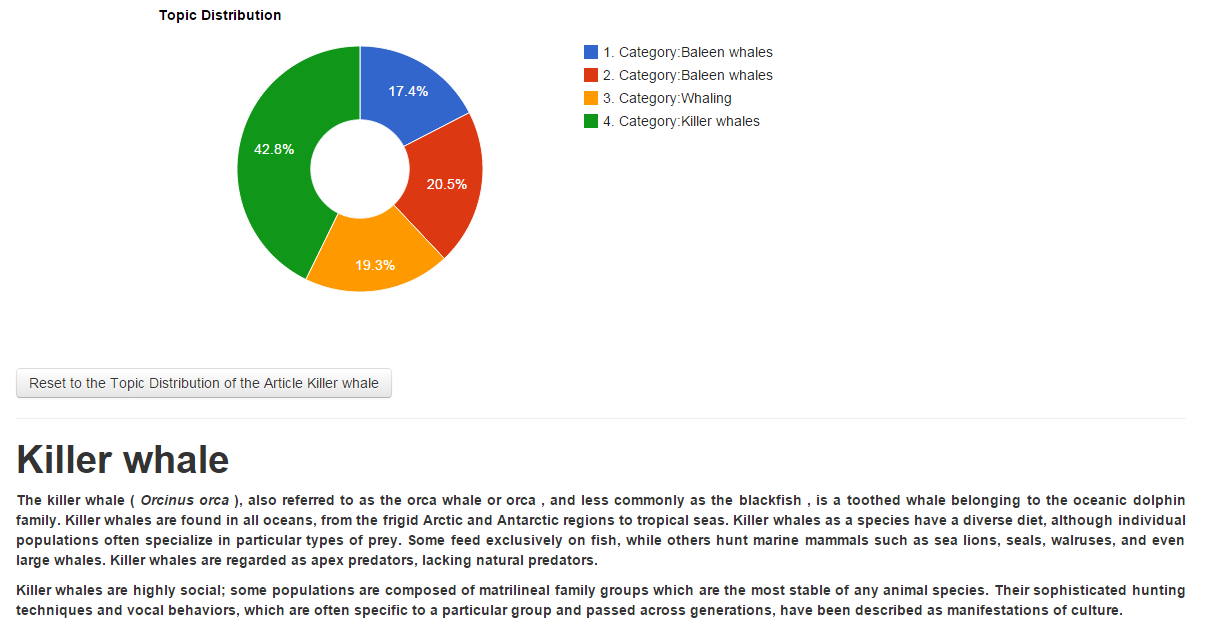
\includegraphics[width=1\textwidth]{images/para_topic_distribution.png}
\caption{Visualizing the topic distribution of the introduction 
section of the Wikipedia article \textit{Killer Whale}. See Figure 
\ref{fig:doc-topic-distribution} for the topic distribution of 
the whole article.}
\label{fig:doc-word-counts}
\end{figure*}

\begin{figure}[htb]\centering 
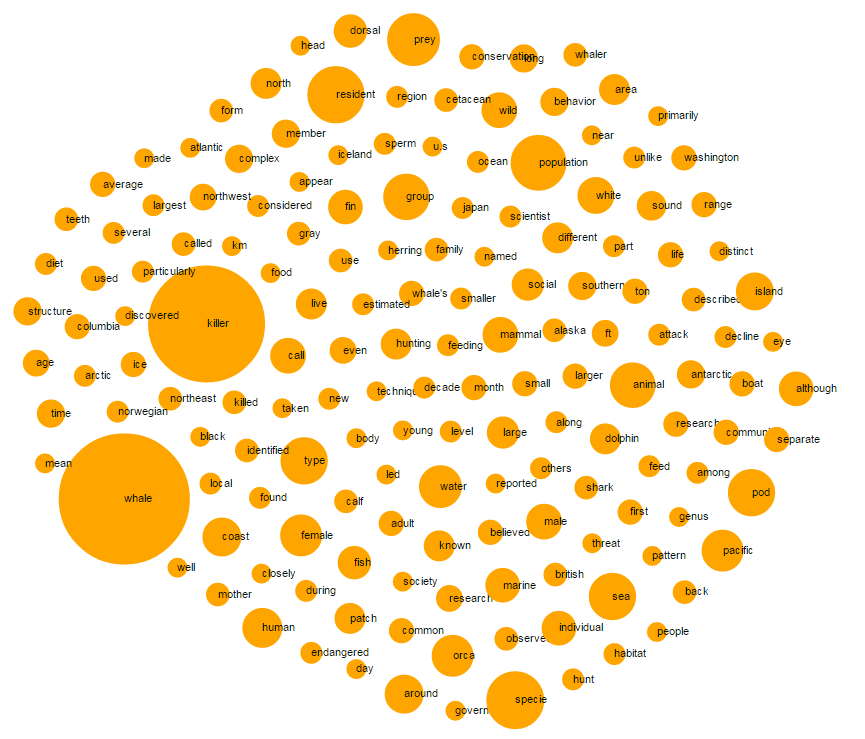
\includegraphics[width=.5\textwidth]{images/doc_tf_bubble_chart.png}
\caption{Visualizing the relative frequencies of terms in the 
Wikipedia article \textit{Killer Whale}. \cpg{I think we need to 
decide whether we should keep this figure in the paper or not.}}
\label{fig:doc-word-counts}
\end{figure}

\paragraph{Graph Explore} One of the most interesting visualizations in the project is the graph explore which allows a user to conceptually drill down a graph of a paper and its citations in a recursive sequence. This is a common method of literature exploration where a user takes up a base paper and then reads up all the papers which have been cited in that base paper. This is recursively performed on the secondary papers also. Though effective, this technique tell the user which ones he should pursue and which ones he should now. The graph explore functionality allows a user to perform this in a more visually appealing and relevant manner. Once a user decides on a base paper and enters it in the system, the system will show a graph representation of its citations which are ranked based on his profile (user model). This will help him pursue the most relevant papers first. Clicking on any secondary paper will open up the graph further and list it's citations ranked taking into account the user model.
